\documentclass[,man,floatsintext]{apa6}
\usepackage{lmodern}
\usepackage{amssymb,amsmath}
\usepackage{ifxetex,ifluatex}
\usepackage{fixltx2e} % provides \textsubscript
\ifnum 0\ifxetex 1\fi\ifluatex 1\fi=0 % if pdftex
  \usepackage[T1]{fontenc}
  \usepackage[utf8]{inputenc}
\else % if luatex or xelatex
  \ifxetex
    \usepackage{mathspec}
  \else
    \usepackage{fontspec}
  \fi
  \defaultfontfeatures{Ligatures=TeX,Scale=MatchLowercase}
\fi
% use upquote if available, for straight quotes in verbatim environments
\IfFileExists{upquote.sty}{\usepackage{upquote}}{}
% use microtype if available
\IfFileExists{microtype.sty}{%
\usepackage{microtype}
\UseMicrotypeSet[protrusion]{basicmath} % disable protrusion for tt fonts
}{}
\usepackage{hyperref}
\hypersetup{unicode=true,
            pdftitle={Designing a Multilingual Copy Task to Measure Typing and Motor Skills in Writing Research},
            pdfauthor={Luuk Van Waes, Mariëlle Leijten, Jens Roeser, Thierry Olive, \& Joachim Grabowski},
            pdfborder={0 0 0},
            breaklinks=true}
\urlstyle{same}  % don't use monospace font for urls
\usepackage{graphicx,grffile}
\makeatletter
\def\maxwidth{\ifdim\Gin@nat@width>\linewidth\linewidth\else\Gin@nat@width\fi}
\def\maxheight{\ifdim\Gin@nat@height>\textheight\textheight\else\Gin@nat@height\fi}
\makeatother
% Scale images if necessary, so that they will not overflow the page
% margins by default, and it is still possible to overwrite the defaults
% using explicit options in \includegraphics[width, height, ...]{}
\setkeys{Gin}{width=\maxwidth,height=\maxheight,keepaspectratio}
\IfFileExists{parskip.sty}{%
\usepackage{parskip}
}{% else
\setlength{\parindent}{0pt}
\setlength{\parskip}{6pt plus 2pt minus 1pt}
}
\setlength{\emergencystretch}{3em}  % prevent overfull lines
\providecommand{\tightlist}{%
  \setlength{\itemsep}{0pt}\setlength{\parskip}{0pt}}
\setcounter{secnumdepth}{0}
% Redefines (sub)paragraphs to behave more like sections
\ifx\paragraph\undefined\else
\let\oldparagraph\paragraph
\renewcommand{\paragraph}[1]{\oldparagraph{#1}\mbox{}}
\fi
\ifx\subparagraph\undefined\else
\let\oldsubparagraph\subparagraph
\renewcommand{\subparagraph}[1]{\oldsubparagraph{#1}\mbox{}}
\fi

%%% Use protect on footnotes to avoid problems with footnotes in titles
\let\rmarkdownfootnote\footnote%
\def\footnote{\protect\rmarkdownfootnote}


  \title{Designing a Multilingual Copy Task to Measure Typing and Motor Skills in Writing Research}
    \author{Luuk Van Waes\textsuperscript{1}, Mariëlle Leijten\textsuperscript{1}, Jens Roeser\textsuperscript{2}, Thierry Olive\textsuperscript{3}, \& Joachim Grabowski\textsuperscript{4}}
    \date{}
  
\shorttitle{Designing a multilingual copy task}
\affiliation{
\vspace{0.5cm}
\textsuperscript{1} Department of Management, University of Antwerp, Belgium\\\textsuperscript{2} Department of Psychology, Nottingham Trent University, United Kingdom\\\textsuperscript{3} Research Centre on Cognition and Learning (CeRCA), CNRS, University of Poitiers, France\\\textsuperscript{4} Institute for Psychology, Leibniz University Hanover, Germany}
\usepackage{csquotes}
\usepackage{upgreek}
\captionsetup{font=singlespacing,justification=justified}

\usepackage{longtable}
\usepackage{lscape}
\usepackage{multirow}
\usepackage{tabularx}
\usepackage[flushleft]{threeparttable}
\usepackage{threeparttablex}

\newenvironment{lltable}{\begin{landscape}\begin{center}\begin{ThreePartTable}}{\end{ThreePartTable}\end{center}\end{landscape}}

\makeatletter
\newcommand\LastLTentrywidth{1em}
\newlength\longtablewidth
\setlength{\longtablewidth}{1in}
\newcommand{\getlongtablewidth}{\begingroup \ifcsname LT@\roman{LT@tables}\endcsname \global\longtablewidth=0pt \renewcommand{\LT@entry}[2]{\global\advance\longtablewidth by ##2\relax\gdef\LastLTentrywidth{##2}}\@nameuse{LT@\roman{LT@tables}} \fi \endgroup}
\usepackage{booktabs}
\usepackage{longtable}
\usepackage{array}
\usepackage{multirow}
\usepackage{wrapfig}
\usepackage{float}
\usepackage{colortbl}
\usepackage{pdflscape}
\usepackage{tabu}
\usepackage{threeparttable}
\usepackage[normalem]{ulem}
\usepackage[utf8]{inputenc}

\authornote{

Correspondence concerning this article should be addressed to Luuk Van Waes, Prinsstraat 13, 2000 Antwerp, Belgium. E-mail: \href{mailto:luuk.vanwaes@uantwerpen.be}{\nolinkurl{luuk.vanwaes@uantwerpen.be}}}



\begin{document}
\maketitle

\hypertarget{method}{%
\section{Method}\label{method}}

As part of a series of research studies using keystroke logging, we collected a corpus of 2066 Dutch copy tasks. Based on this corpus, we will first present some general information to characterize this data set. Second, we will present a Bayesian analysis of inter-keystroke intervals using mixed effects and mixture models that aims at characterizing the distributions of the copy-task components and their differences between all copy-task components, how random effects may be used as a diagnositc tool and additionally the test-retest reliability of the copy-task components.

\hypertarget{participants}{%
\subsection{Participants}\label{participants}}

For the present analysis we used the Dutch corpus of copy-task data. The data were collected from 1662 participants (1107 females, 495 males, 80 unknowns) aged between 13 and 83 years old (median=21 years; \(SD\)=11.81) in the context of various research projects, research courses and training schools. As most of these studies took place at secondary schools or universities this explains why age groups are not equally represented: 78.94\% of the participants are 23 or younger.

The distribution of participants' age and their inter-keystroke intervals can be found in Figure \ref{fig:age}. This distribution is illustrated in different colours for each copy-task component illustrating the relationship between copy-task components and age. For each component we observe a nonlinear positive relationship between age and keystroke latencies (Bosman, 1993; Van Waes, Leijten, Mariën, \& Engelborghs, 2017). From handwriting research we know that automaticity is reached at about the age of fifteen (for an overview see, for instance, Graham, 1997; Graham \& R. Harris, 2000; Medwell \& Wray, 2014). Our data shows that typing performance is the fastest between 21 and 30. From the age of 30 onward typing skills seem to gradually decrease. At the age of 50 participants are on average slower than the 20 year olds. But even in the latter age group it is important to notice that typing skills might differ considerably. Interestingly, this graph suggests different functions for lexical compared to non-lexical tasks. Lexical tasks show an early speed-up that is not seen in the non-lexical tasks for this age range.

\begin{figure}[!h]

{\centering \includegraphics{ct_files/figure-latex/unnamed-chunk-2-1} 

}

\caption{\label{fig:age}Distirbution of age groups and the relationship between age and inter-keystroke intervals (IKIs). For visuallisation data were aggregated on participant-level and IKIs were capped at 3,500 msecs. Lexical tasks were indicated by solid lines and non-lexical tasks were displayed with dashed lines. Both axes are log-scale.}\label{fig:unnamed-chunk-2}
\end{figure}

\hypertarget{materials}{%
\subsection{Materials}\label{materials}}

The copy-task corpus contains currently 1447310 inter-keystroke intervals (per logfile: \(M\)=700.54; \(SD\)=78.56) characterized by a set of variables: inter-keystroke interval (IKI) transition time (in msecs), copy-task component and trial in which they were produced as well as frequency characteristics, hand combination needed to produce the bigram, adjacency and repetition. The data are available in both an XML and a CSV-output file using the Inputlog 8 copy task analysis. The XML file contains aggregated analyses at the logfile level offering different perspectives to the copy task data (e.g.~frequency, hand combinations, repetition, adjacency) at different levels (e.g.~global, targeted bigrams, component and trial level). Moreover, time and trial filters are also applied and apart from means, medians and standard deviations. Also geometric means and confidence intervals are presented. The CSV file is a non-aggregated output containing a full list of bigrams typed enriched with information about the component (and trial) in which they were composed, their IKI duration, and characteristics (see perspectives above).

\(R\)-scripts and datasets are available on Github (URL) and can be used for reproducing and extending the presented analysis for further investigation involving the copy-task data.

\hypertarget{data-analysis}{%
\subsection{Data analysis}\label{data-analysis}}

The aim of this analysis is to provide estimates of the distribution parameters underlying each copy-task component. This is achieved in two ways: First, we determined inferential estimates of the population parameters, the mean \(\mu\) and the variance \(\sigma^2\), of each copy-task component. Second, we estimated probability distributions of the differences between the inter-keystroke intervals of all copy-task components. Third, we extended this analysis to evaluate typing performance of individual typists and the test-retest reliability of the copy-task.

The inter-keystroke intervals, the duration between two consecutive keystrokes, were analysed in Bayesian linear mixed effects models (see e.g. Gelman \& Hill, 2007; Gelman et al., 2014; Kruschke, 2014; Lambert, 2018; McElreath, 2016), using the probabilistic programming language Stan (Carpenter et al., 2016; Hoffman \& Gelman, 2014; Stan Development Team, 2015a, 2015b). This approach provides and adequate framework to handle unequal variance and unequal numbers of observations (Quené \& Van den Bergh, 2004, 2008; Van Waes, Leijten, \& Quinlan, 2010). The Bayesian framework used in this analysis provides statistically inferred (i.e.~posterior) quantities that have a fundamentally different theoretical interpretation than frequentist quantifies (see for detailed discussions Kruschke, 2014; Lambert, 2018; McElreath, 2016; Nicenboim \& Vasishth, 2016).\footnote{A frequentist analysis using and the \(R\) package lme4 (Bates et al., 2015b) for linear mixed effects models and a comparison to Bayesian linear mixed effects model can be found in Appendix \ref{comparing-bayesian-and-frequentist-models}.}

The Bayesian linear mixed effects model was extended to a mixture model (Farrell \& Lewandowsky, 2018; Gelman et al., 2014; Vasishth, Chopin, Ryder, \& Nicenboim, 2017). This extension was used to map the data to the assumed underlying cognitive process that generates these data. As highlighted in the introduction of this paper, keystroke data as well as many other lower-level tasks are a combination of different cognitive processes which cascade from higher into lower levels of representation. Mixture models assume that the underlying data generating process is a combination of Gaussians (i.e.~normal distributions). In contrast, statistical methods such as analysis of variance (ANOVA) and \(t\)-tests but also linear regression models assume the data to come from a single underlying normal distribution. While regression models estimate one population mean \(\mu\) and variance \(\sigma^2\) from the data, a mixture model with two mixture components would estimate \(\mu\) and \(\sigma^2\) for two component involved in the underlying data generating process. This is achieved by introducing an additional (latent) model parameter -- the mixing proportions \(\theta\) -- which captures the probability to which data are attributed to either distribution.

This analysis focuses specifically on providing a model that is capable of accounting for the mixture of cognitive processes involved in copy-typing. Inter-keystroke intervals may reflect processes on various levels of encoding. For example, Baaijen, Galbraith, and Glopper (2012) used a mixture model approach to analyse pauses in text writing and found a combination of three Gaussians with a mixing proportion of .65 with a mean pause duration of 330 msecs which the attributed to for word retrieval, a proportion of .26 around 735 msecs for phrase boundaries, and .09 for higher level processes (e.g.~planning, reflection) with a mean pause durations of 2697 msecs. In other words pausing in text writing is a combination of three processes that are represented in 65\%, 26\% and 9\% in the data, respectively. Copy-typing in our example is similar to the extent that it involves a mixture of cognitive processes. For example, copy-typists need to visually encode the target string, buffer its representation in memory, activate the relevant motor code, execute the keystrokes and update the memory representation of the target string. This may or may not involve revision and linguistic processing.

The advantages of Bayesian data analysis for hypothesis testing are well documented in the literature (Dienes, 2014; Kruschke, 2014; Kruschke, Aguinis, \& Joo, 2012; Kruschke \& Liddell, 2018; Nicenboim \& Vasishth, 2016; Sorensen, Hohenstein, \& Vasishth, 2015). An attractive properties of Bayesian statistics is the fact that the posterior / inferred quantities are associated with a probability distribution. In other words, Bayesian inference allows us to determine the most probable value indicating the difference between two copy-task components and the probability range round this value. The former estimate is called the \textit{maximum a posteriori}, the most probable parameter estimate. Along with this estimate we can determine the shortest interval containing 95\% of the posterior probability mass. This interval is called the 95\% Highest Posterior Density Interval (HPDI). Bayesian HPDIs, probability, percentile intervals, and credible intervals provide a probability range in which the true parameter value lies with the highest certainty. HPDIs are typically used for non-symmetric posteriors (Hyndman, 1996; Liu, Gelman, \& Zheng, 2015), for example, bimodal or skewed posterior distributions. Although frequentist confidence intervals are often mistake to have similar properties, frequentist quantities do generally not provide any probability information about the inferred parameter value (see Hoekstra, Morey, Rouder, \& Wagenmakers, 2014; Morey, Hoekstra, Rouder, Lee, \& Wagenmakers, 2015) (for more details see Appendix \ref{comparing-bayesian-and-frequentist-models}).

All reported models include random intercepts for participants and bigrams to account for individual differences between both participants' typing ability and differences between individual bigrams (e.g.~frequency, hand combination, adjacency). To avoid over-parametrisation of the models (see Baayen, Davidson, \& Bates, 2008; Bates et al., 2015a) we did not include random by-participants slopes for copy-task components, unless stated differently.\footnote{All models were fitted with weakly informative regulating priors (see Lambert, 2018). 6,000 iterations (3,000 warm-up) were run for 3 Markov chain Monte Carlo chains. Model convergence was tested via the Rubin-Gelman statistic (Gelman \& Rubin, 1992), traceplots and cross-validation (Vehtari, Gelman, \& Gabry, 2015, 2017).}

\hypertarget{data-preprocessing}{%
\subsection{Data preprocessing}\label{data-preprocessing}}

For this analysis, the keystroke data were minimally trimmed. Missing data (0.01\%) and inter-keystroke intervals equal to zero (0.02\%) were removed as well as non-targeted bigrams (4.25\%).\footnote{The rationale for this decision can be found in Appendix \ref{data-trimming}} The overall median score for correctly typed bigrams was 96.35\% (\(IQR\)=3.03), and varied between a minimum of 87.13\% and a maximum of 96\% across copy-task components.

For the following analysis data were aggregated across repetitions rendering one inter-keystroke interval per letter combination (i.e.~bigram) per participant. The analysis was performed on a random subset of 500 participants.

\hypertarget{results}{%
\section{Results}\label{results}}

\hypertarget{mixture-models-of-inter-keystroke-intervals}{%
\subsection{Mixture models of inter-keystroke intervals}\label{mixture-models-of-inter-keystroke-intervals}}

Figure \ref{fig:descr} shows boxplots of the inter-keystroke intervals with the individual data as jittered dots. The distributions show both the central tendency and dispersion of the data. More difficult tasks appear to be associated with longer inter-keystroke intervals. The non-lexical tasks demarcate the limits of the inter-keystroke interval. The purely motoric tapping component shows very short keystrokes and the Consonant task involving memory storage and eye-hand coordination shows particularly long keystroke intervals. The lexical components show a clear difference between the LF bigram task on the one side and the HF bigrams and Sentence task on the other side.

\begin{figure}[!h]

{\centering 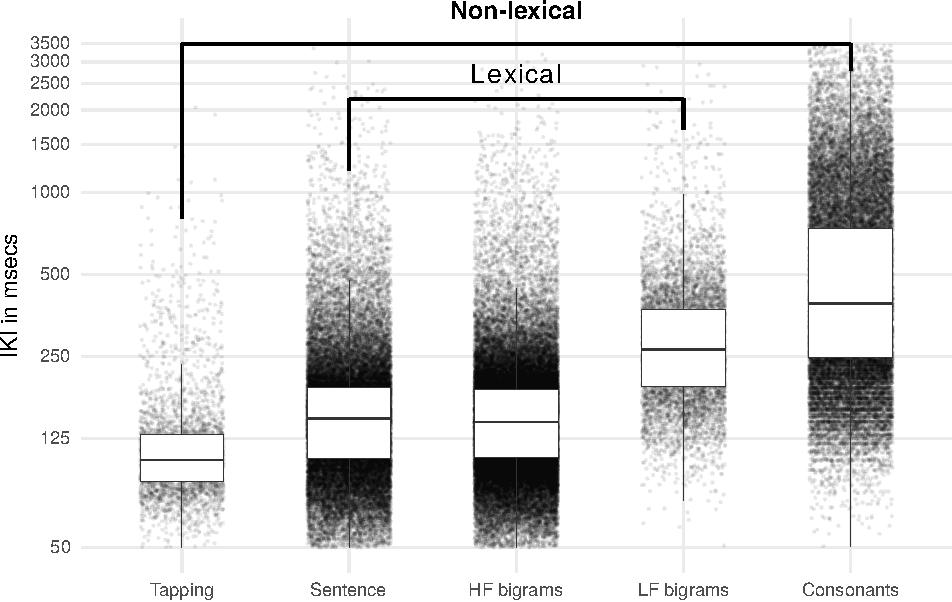
\includegraphics{ct_files/figure-latex/fig2-1} 

}

\caption{\label{fig:descr}Boxplots of the inter-keystroke intervals (IKI) for each copy-task component of the entire corpus. For visualisation, the data were capped at 3,500 msecs and shown on a log scale.}\label{fig:fig2}
\end{figure}

In addition to the differences between components shown in Figure \ref{fig:descr}, there are clear differences in the variance between the components. In particular the Consonant task shows a wide dispersion. The dark area around the boxplots for the Sentence and HF bigram task illustrates a dense distribution of the inter-keystroke intervals around a centre. While most components seem to be associated with a specific variance, the sentence copying task and the HF bigram task show similar distributions. In other words, the variance of the majority of copy-task components is unequal (i.e.~heteroscedastisciy).

Linear mixed effects models (as well as ANOVAs and \(t\)-tests) assumed equality of variance (i.e.~homoscedasticity) between the different conditions. In other words, the variance of each copy-task component should be approximately the same. We compared the fit of 5 Bayesian models to (1) fit the data of the copy-task components, (2) evaluate the equality of variance and (3) test whether the data in each component arise from a mixture of normal distributions.

First we fitted a linear mixed effects model with an intercept term only (a null model). This model was compared to a model with copy-task component as fixed effect. A comparison of these two models allows us to determine the predictive power of copy-task component. The heteroscedasticity assumption as implemented in a linear mixed effects model that assumes that each copy-task component has its own population mean \(\mu\) and its own variance parameter \(\sigma^2\). This assumption was carried over into the mixture models. Mixture models were fitted with two and three underlying components. The mixture models with two underlying distributions was fitted was constrained such that the distribution with the larger centre (mean) has a larger variance. The reason for this was that it is well know that larger values are associated with a larger variances for both response-time data in particular (Wagenmakers \& Brown, 2007) and human motor bahaviour in general (Schöner, 2002; Wing \& Kristofferson, 1973). A last model was fitted with three mixture components of which the new additional component was constrained to capture extremely short inter-keystroke intervals.

To compare the fit of the different models we used leave-one-out cross-validation which allows to test the predictive ability of models and penalizes models with more parameters (see Farrell \& Lewandowsky, 2018; Lambert, 2018; Lee \& Wagenmakers, 2014; McElreath, 2016). We determined this out-of-sample predictive performance via Pareto smoothed importance-sampling leave-one-out cross-validation (PSIS-LOO) (Vehtari et al., 2015, 2017). This predictive performance was estimated as the sum of the expected log pointwise predictive density (\(\widehat{elpd}\)) and can be found in Table \ref{tab:fit}. A higher \(\widehat{elpd}\) indicates better predictive performance. The difference between the predictive quality of the best fitting model compared to the remaining models was expressed as \(\Delta\widehat{elpd}\). A negative difference \(\Delta\widehat{elpd}\) indicates that the predictive performance of a model is lower compared to the best fitting model.

\begin{table}[t]

\caption{\label{tab:unnamed-chunk-4}\label{tab:fit}Predictive performance of five Bayesian models, three Bayesian linear mixed effects models (BLMM) and two Mixture of Gaussians (MoG) models with \textit{K} mixture components. $\widehat{elpd}$ is the expected log pointwise predictive density. The model fit was ordered starting with the model with the highest predictive performance on the top. Differences in model fit $\Delta\widehat{elpd}$ (\textit{SE}=standard error) are shown with reference to the model with the highest predictive performance.}
\centering
\fontsize{11}{13}\selectfont
\begin{tabu} to \linewidth {>{\raggedright\arraybackslash}p{4.5cm}>{\raggedleft\arraybackslash}p{2cm}>{\raggedleft\arraybackslash}p{2cm}>{\raggedleft\arraybackslash}p{2cm}>{}p{2cm}}
\toprule
Model & $\Delta\widehat{elpd}$ & SE & $\widehat{elpd}$\\
\midrule
MoG (\textit{K}=3) & 0.00 & 0.00 & -227275.0\\
MoG (\textit{K}=2) & -64.37 & 15.67 & -227339.4\\
BLMM (unequal variance) & -1192.86 & 80.52 & -228467.9\\
BLMM (equal variance) & -4368.63 & 121.59 & -231643.7\\
BLMM (intercept-only) & -4618.42 & 123.91 & -231893.5\\
\bottomrule
\end{tabu}
\end{table}

Both mixture models showed a higher predictive performance than the linear mixed effects models with an increase in predictive performance of around \(\Delta\widehat{elpd}\)=1,000 compared to the best fitting linear mixed effects model. Adding an additional mixture component to the mixture model with three mixture components renders a comparably negligible gain (\(\Delta\widehat{elpd}=\)-64.37, \textit{SE}=15.67). Therefore, we will use use the model with two mixture components for inference. The Bayesian linear mixed effects model with unequal variance for each copy-task component rendered a higher predictive performance compared to the equal variance standard linear mixed effects models. The lowest predictive performance was observed for the intercept-only model. Including copy-task component as model parameter improved the predictive performance of the model. Allowing varying variance parameters increases the predictive performance of the models as well as the addition of mixture components.

The parameter estimates for each copy-task component are summarised in Table \ref{tab:musum}.
The most probable parameter estimate (i.e. \textit{maximum a posteriori} {[}MAP{]}) and 95\% HPDIs for each copy-task component. \(\hat{\mu}\) indicates the distribution of probable parameter values for each component. Values are shown for each each mixture component.

\begin{table}[t]

\caption{\label{tab:unnamed-chunk-5}\label{tab:musum}Parameter estimates for each copy-task component. Shown are the \textit{maximum a posteriori} (MAP), the most probable parameter value, and the lower (2.5\%) and upper bound (97.5\%) of the 95\% HPDI (all in msecs). Values for the mixture component of shorter values are shown in the $\hat{\mu}_1$ column, values for the component of longer values are shown in the $\hat{\mu}_2$ column.}
\centering
\fontsize{11}{13}\selectfont
\begin{tabu} to \linewidth {>{\centering\arraybackslash}p{2.5cm}>{\raggedright\arraybackslash}p{3cm}>{\raggedleft\arraybackslash}p{2.5cm}>{\raggedleft\arraybackslash}p{2.5cm}>{\raggedleft\arraybackslash}p{2.5cm}>{}p{2.5cm}}
\toprule
Mixture component & Copy-task component & MAP & 2.5\% HPDI & 97.5\% HPDI\\
\midrule
 & Tapping & 127.28 & 80.51 & 179.97\\

 & Sentence & 156.18 & 144.96 & 169.19\\

 & HF bigrams & 166.27 & 154.63 & 180.41\\

 & LF bigrams & 251.29 & 187.60 & 336.47\\

\multirow{-5}{2.5cm}{\centering\arraybackslash $\hat{\mu}_1$} & Consonants & 238.12 & 216.97 & 256.74\\
\cmidrule{1-5}
 & Tapping & 187.10 & 113.52 & 282.58\\

 & Sentence & 183.98 & 169.65 & 200.70\\

 & HF bigrams & 169.78 & 157.29 & 185.99\\

 & LF bigrams & 355.83 & 234.56 & 595.35\\

\multirow{-5}{2.5cm}{\centering\arraybackslash $\hat{\mu}_2$} & Consonants & 377.06 & 344.72 & 409.95\\
\bottomrule
\end{tabu}
\end{table}

For a visualisation of Table \ref{tab:musum}, including the mixing proportion see Figure \ref{fig:mog}. The mixing proportion is indicated as \(\theta\) which can be understood as the probability of data to be part of a mixture component. This mixing proportion ranges from \(>\) 0 to \(<\) 1. The mixing proportion of the mixture component \textit{K}\(_2\) is indicated as \(\hat{\theta_2}\) and indicates the probability of data belonging to the distribution \(\hat{\mu_2}\). As the model is constrained to be bimodal, \(\hat{\theta_2}\) is equal to \(1-\hat{\theta_1}\), where \(\theta_1\) is the mixing proportion of the mixture model \textit{K}\(_1\).

\begin{figure}[!h]

{\centering \includegraphics{ct_files/figure-latex/fig3-1} 

}

\caption{\label{fig:mog}Parameter estimates of the mixture model for each copy-task component. Shown as dots are the most probable parameter estimate and 95\% HPDIs as error bars. The mixture component is indicates as subscripts. $\hat\mu$ indicates the parameter estimates, and $\hat\theta_2$ the mixing proportion.}\label{fig:fig3}
\end{figure}

The mixing proportion \(\hat\theta_2\) is relatively small for most components. In other words, the majority of the posterior probability lies in one mixture component. This smaller proportion may be attributed to occasional pausing or possibly slower initial keystrokes. However, for the Consonant task, the mixing proportion of \(\hat\theta_2\) is 0.69 (95\% HPDI: 0.65, 0.72). Thus 69\% of the bigram data in the Consonant task are attributed to a distribution of longer keystroke intervals.

The estimates of the parameter value \(\hat\mu\) show two groups; the first comprises the Tapping task, Sentence typing and HF bigrams, the second comprises the LF bigrams and the Consonant task. This applies to both distributions, \textit{K}\(_1\) and \textit{K}\(_2\). The HPDIs indicate that certainty about the parameter estimate is lower in the Tapping task and the Consonant task than in the remaining three tasks indicating some variability between fast and slow inter-keystroke intervals.

The parameter estimates of the linear mixed model are compared to the parameter estimates of each mixture component in Figure \ref{fig:moglmm}. The mixing proportion \(\hat\theta_2\) of \(\hat\mu_2\) and their 95\% HPDIs are shown on the panel labels.

\begin{figure}[!h]

{\centering \includegraphics{ct_files/figure-latex/fig4-1} 

}

\caption{\label{fig:moglmm}Comparison of parameter estimates of the Bayesian linear mixed effects model (BLMM) and the mixture model showing the most probable parameter estimate $\hat\mu$ with HPDI for both components indicated by subscripts. Parameter estimates are shown for all copy-task components.}\label{fig:fig4}
\end{figure}

The parameter estimate \(\hat\mu_1\) of the mixture model is similar to the estimates of the Bayesian linear mixed effects model in the Tapping task, the Sentence and the HF bigrams task, and the LF bigram task. In the Tapping, Sentence and LF bigram task, \(\hat\mu_2\) accounts for occasional slowdowns. In the HF bigrams task, both mixture components are consistent with the parameter estimates of the linear mixed effects models. However, the Sentence typing task and, in particular, the Consonant task show shorter inter-keystroke intervals \(\hat\mu_1\) compared to the previous estimates while \(\hat\mu_2\) is longer. This indicates that the previous estimates where higher because of a subset of longer values. This pattern was the strongest in the Consonant task in which the two parameter estimates \(\hat\mu_1\) and \(\hat\mu_2\) are more distinct representing about 30\% and 70\% of the inter-keystroke intervals, respectively.

The differences between inter-keystroke intervals were assessed in pairwise comparisons between all copy-task components. The most probable difference estimate with 95\% HPDI can be found in Figure \ref{fig:comps} with the compared components shown on the left and right side. To comparability the differences are shown for both parameter estimates \(\hat\mu\) of the mixture model in the upper panel and the differences in \(\hat\theta_2\) can be found in the lower panel. Numbers above the intervals show \textit{P}(\(\Delta\hat\mu<0\)), the probability that the posterior difference between the copy-task components is smaller than zero. Small posterior differences indicate a high probability that there is a difference larger than zero.

\begin{figure}[!h]

{\centering \includegraphics{ct_files/figure-latex/fig5-1} 

}

\caption{\label{fig:comps}Difference in inter-keystroke intervals between copy-task components shown for mixture components $\hat\mu$ and mixing proportion $\hat{\theta}_2$ with 95\% HPDIs. Numbers in the graph shown the posterior probability of the difference being smaller than zero \textit{P}($\Delta\hat\mu<0$). Values of \textit{P}($\Delta\hat\mu<0$)<.001 or >.999 were omitted.}\label{fig:fig5}
\end{figure}

Figure \ref{fig:comps} shows that there are consistent differences between inter-keystroke intervals across the majority of copy-task components. The magnitude of the difference and its variability differs. There is a small but consistent difference between the Sentence and HF bigram task. The differences between the Consonant task and the Tapping, HF bigrams, and Sentence task have a large magnitude. Differences between the LF bigram task and the Tapping, Sentence, and HF bigram task are consistently above zero but variable in its magnitude. The differences between the Tapping task and HF bigrams and the Sentence component are small, show little variability but show some proportional of differences in the opposite direction. The inconsistent difference between the LF bigram task and the Consonants component observed in the linear mixed effects model disappear in the mixture model analysis. Large component differences in the mixing proportion \(\hat\theta_2\) can be seen for comparisons that involve the Consonant task. The consonant task exhibits a larger mixing proportion \(\hat\theta_2\) compared to the remaining copy-task components.

\hypertarget{individual-variance}{%
\subsection{Individual variance}\label{individual-variance}}

Linear mixed effects models allow us to estimate varying intercepts for each participants. The parameter estimates for each individual can be used to identify those individuals that are relatively fast or slow typists compared to the reminder of the sample. In other words, we can use this tool to test the typing performance and isolate individuals that vary from the remainder of the sample. Figure \ref{fig:inddiff} shows a caterpillar plot for the deviation estimates for each participants.

\begin{figure}[!h]

{\centering \includegraphics{ct_files/figure-latex/unnamed-chunk-7-1} 

}

\caption{\label{fig:inddiff}Participant deviation from the model intercept. Each errorbar represents the 95\% HPDI for one participant. Participants with large deviations (MAP $>$ 3 $\times$ SD) were labelled with their participant ID.}\label{fig:unnamed-chunk-7}
\end{figure}

For each participant we plotted the 95\% HPDI interval showing the deviation from the overall intercept marked by the dashed line intercepting at zero. As the distribution of these deviations is normal, it allows us to identify those individuals that are relatively slow or fast. In Figure \ref{fig:inddiff} relatively fast individuals are shown on the left side and relatively slow individuals are shown on the right. Those HPDIs that did not fall into the normal distribution of those deviations were labelled with the participants' ID. For example, the slowest typist in the sample shown were participants 236 and 437.

The same logic can be applied to isolate individuals with difficulty in certain copy-task components. This can be used to identify individuals with specific difficulty on the motor level (Tapping), in lexical typing tasks (HF/LF bigrams, Sentence task), or tasks that involve eye-hand coordination and a memory component (Consonant task). To illustrate how we can use the copy-task as a diagnostic tool we focused on a group that typically shows more difficulty. We selected the 2.5\% oldest participants in the copy-task corpus (\textit{N}=79, 32 males, 48 females; median age = 67 years, range: 60, 83). We fitted a Bayesian linear mixed effects model as described before with intercept as fixed effect and random intercepts for bigrams and participants with by-participants slopes for copy-task component. The results of this model can be found in Figure \ref{fig:agediff}. Figure \ref{fig:agediff} shows the typing deviation from the overall intercept (shown as dashed line) for each participant plotted against age. Those individuals that showed a relatively slow performance were labelled with their participant ID.

\begin{figure}[!h]

{\centering \includegraphics{ct_files/figure-latex/unnamed-chunk-9-1} 

}

\caption{\label{fig:agediff}Participant deviation from the overall intercept with 95\% HPDIs. Age is shown on the x-axis and indicate as colour (i.e. darker colour indicates higher age). For each component, participant IDs are shown for individuals that show slower responses compared to the remainder of the sample (MAP $>$ 3 $\times$ SD).}\label{fig:unnamed-chunk-9}
\end{figure}

Figure \ref{fig:agediff} illustrates that participant 74 shows more difficulty in most copy-task components, except the Tapping task. In contrast, participants 10, 18, and 36 show difficulty in the Tapping task but in none of the other copy-task components. Participants 14 shows difficulty in the Sentence and HF bigrams task only. Participant 6 shows difficulty in the LF bigrams and Consonant task. Participant 8 shows difficulty across all copy-task components. In other words, we can detect participants that have difficulty related to the properties of certain copy-task components.

\hypertarget{test-retest-reliability}{%
\subsection{Test-retest reliability}\label{test-retest-reliability}}

Stability of the measures was assessed in a test-retest design: 245 participants completed the copy task twice with a time lag interval of at least one week (195 males, 45 females; median age = 22 years, range: 15, 73).

We used a Bayesian linear mixed effects model, specified as previously described, to evaluate the whether participants were faster during the completion of the second session. We added the coefficient \(\delta\) to the model to capture the changes in inter-keystroke intervals in the second session. The estimate for the anticipated speed-up effect was obtained for each copy-task component separately.

We found speed-up effects of \(\hat\delta\) = -10.88 msecs for the Tapping component (95\% HPDI: -20.34, -3.24), \(\hat\delta\) = -12.17 msecs (95\% HPDI: -23.99, -3.98) for LF bigrams and for the Consonant task \(\hat\delta\) = -9.01 msecs (95\% HPDI: -14.65, -3.67). The speed-up effect for the Sentence task (\(\hat\delta\) = -2.00 msecs; 95\% HPDI: -4.60, 0.23) and HF bigrams (\(\hat\delta\) = -0.98 msecs; 95\% HPDI: -3.04, 1.19) has a small magnitude and the HPDIs include 0 as possible parameter value. For the other components, the speed-up effect is systematic and has a very small magnitude.

These differences are too small to suggest a strategic change in participants' responses but seems to relate to task familiarity. This is illustrated in Figure \ref{fig:retestgroup}. Although there is a systematic speed-up in some copy-task components, the effect does not change the overall pattern of the copy-task components.

\begin{figure}[!h]

{\centering \includegraphics{ct_files/figure-latex/unnamed-chunk-12-1} 

}

\caption{\label{fig:retestgroup}Statistically inferred parameter values $\hat{\mu}$ for each session shown by copy-task component. Dots indicate the most probable parameter value and errorbars show 95\% HPDIs.}\label{fig:unnamed-chunk-12}
\end{figure}

These results confirm the reliability of the copy-task. For each of the copy-task components the general pattern observed in inter-keystroke intervals was reproduced in a second session in spite of a systematic but small typing advantage in the second session. This can be explained in terms of hesitations that might be related to accommodation to the novelty of the copy-task environment.

\hypertarget{summary}{%
\section{Summary}\label{summary}}

In this analysis we showed how linear mixed effects models and an extension to mixture models can be used evaluate the distribution characteristics of each copy-task component and their respective differences. In particular, we showed that copy-typing is to some extent a mixture process involving more than one cognitive component. Further, we show how a random effects analysis of the copy-task data can be used as a diagnostic tool, to isolate individuals with specific difficulties. Lastly, we demonstrated the test-retest reliability of the copy-task showing that although there is a systematic speed-up effect for individuals performing in a second session of the copy-task, the difference does not affect the overall pattern across copy-task components.

\hypertarget{references}{%
\section{References}\label{references}}

\begingroup
\setlength{\parindent}{-0.5in}
\setlength{\leftskip}{0.5in}

\hypertarget{ref}{}

\endgroup

\hypertarget{refs}{}
\leavevmode\hypertarget{ref-baaijen2012keystroke}{}%
Baaijen, V. M., Galbraith, D., \& Glopper, K. de. (2012). Keystroke analysis: Reflections on procedures and measures. \emph{Written Communication}, \emph{29}(3), 246--277.

\leavevmode\hypertarget{ref-baa08}{}%
Baayen, R. H., Davidson, D. J., \& Bates, D. M. (2008). Mixed-effects modeling with crossed random effects for subjects and items. \emph{Journal of Memory and Language}, \emph{59}(4), 390--412.

\leavevmode\hypertarget{ref-bates2015parsimonious}{}%
Bates, D. M., Kliegl, R., Vasishth, S., \& Baayen, R. H. (2015a). Parsimonious mixed models. \emph{arXiv Preprint arXiv:1506.04967}.

\leavevmode\hypertarget{ref-bates2015}{}%
Bates, D. M., Mächler, M., Bolker, B., \& Walker, S. (2015b). Fitting linear mixed-effects models using lme4. \emph{Journal of Statistical Software}, \emph{67}(1), 1--48. \url{https://doi.org/10.18637/jss.v067.i01}

\leavevmode\hypertarget{ref-bosman1993age}{}%
Bosman, E. A. (1993). Age-related differences in the motoric aspects of transcription typing skill. \emph{Psychology and Aging}, \emph{8}(1), 87--102.

\leavevmode\hypertarget{ref-carpenter2016stan}{}%
Carpenter, B., Gelman, A., Hoffman, M. D., Lee, D., Goodrich, B., Betancourt, M., \ldots{} Riddell, A. (2016). Stan: A probabilistic programming language. \emph{Journal of Statistical Software}, \emph{20}.

\leavevmode\hypertarget{ref-dienes2014using}{}%
Dienes, Z. (2014). Using Bayes to get the most out of non-significant results. \emph{Frontiers in Psychology}, \emph{5}(781), 1--17.

\leavevmode\hypertarget{ref-farrell2018computational}{}%
Farrell, S., \& Lewandowsky, S. (2018). \emph{Computational modeling of cognition and behavior}. Cambridge University Press.

\leavevmode\hypertarget{ref-gelman2014}{}%
Gelman, A., Carlin, J. B., Stern, H. S., Dunson, D. B., Vehtari, A., \& Rubin, D. B. (2014). \emph{Bayesian data analysis} (3rd ed.). Chapman; Hall/CRC.

\leavevmode\hypertarget{ref-gel07}{}%
Gelman, A., \& Hill, J. (2007). \emph{Data analysis using regression and multilevel/hierarchical models}. Cambridge: Cambridge University Press.

\leavevmode\hypertarget{ref-gelman1992}{}%
Gelman, A., \& Rubin, D. B. (1992). Inference from iterative simulation using multiple sequences. \emph{Statistical Science}, \emph{7}(4), 457--472.

\leavevmode\hypertarget{ref-graham1997executive}{}%
Graham, S. (1997). Executive control in the revising of students with learning and writing difficulties. \emph{Journal of Educational Psychology}, \emph{89}(2), 223--234.

\leavevmode\hypertarget{ref-graham2000role}{}%
Graham, S., \& R. Harris, K. (2000). The role of self-regulation and transcription skills in writing and writing development. \emph{Educational Psychologist}, \emph{35}(1), 3--12.

\leavevmode\hypertarget{ref-hoekstra2014robust}{}%
Hoekstra, R., Morey, R. D., Rouder, J. N., \& Wagenmakers, E.-J. (2014). Robust misinterpretation of confidence intervals. \emph{Psychonomic Bulletin \& Review}, \emph{21}(5), 1157--1164.

\leavevmode\hypertarget{ref-hoffman2014no}{}%
Hoffman, M. D., \& Gelman, A. (2014). The No-U-Turn sampler: Adaptively setting path lengths in Hamiltonian Monte Carlo. \emph{Journal of Machine Learning Research}, \emph{15}(1), 1593--1623.

\leavevmode\hypertarget{ref-hyndman1996computing}{}%
Hyndman, R. J. (1996). Computing and graphing highest density regions. \emph{The American Statistician}, \emph{50}(2), 120--126.

\leavevmode\hypertarget{ref-kruschke2014doing}{}%
Kruschke, J. K. (2014). \emph{Doing bayesian data analysis: A tutorial with R, JAGS, and Stan} (2nd ed.). Academic Press.

\leavevmode\hypertarget{ref-kruschke2012time}{}%
Kruschke, J. K., Aguinis, H., \& Joo, H. (2012). The time has come: Bayesian methods for data analysis in the organizational sciences. \emph{Organizational Research Methods}, \emph{15}(4), 722--752.

\leavevmode\hypertarget{ref-kruschke2018bayesian}{}%
Kruschke, J. K., \& Liddell, T. M. (2018). The Bayesian New Statistics: Hypothesis testing, estimation, meta-analysis, and power analysis from a bayesian perspective. \emph{Psychonomic Bulletin \& Review}, \emph{25}(1), 178--206.

\leavevmode\hypertarget{ref-lambert2018student}{}%
Lambert, B. (2018). \emph{A student's guide to Bayesian statistics}. Sage.

\leavevmode\hypertarget{ref-lee2014bayesian}{}%
Lee, M. D., \& Wagenmakers, E.-J. (2014). \emph{Bayesian cognitive modeling: A practical course}. Cambridge University Press.

\leavevmode\hypertarget{ref-liu2015simulation}{}%
Liu, Y., Gelman, A., \& Zheng, T. (2015). Simulation-efficient shortest probability intervals. \emph{Statistics and Computing}, \emph{25}(4), 809--819.

\leavevmode\hypertarget{ref-mcelreath2016statistical}{}%
McElreath, R. (2016). \emph{Statistical rethinking: A bayesian course with examples in R and Stan}. CRC Press.

\leavevmode\hypertarget{ref-medwell2014handwriting}{}%
Medwell, J., \& Wray, D. (2014). Handwriting automaticity: The search for performance thresholds. \emph{Language and Education}, \emph{28}(1), 34--51. \url{https://doi.org/10.1080/09500782.2013.763819}

\leavevmode\hypertarget{ref-morey2015Fallacy}{}%
Morey, R. D., Hoekstra, R., Rouder, J. N., Lee, M. D., \& Wagenmakers, E.-J. (2015). The fallacy of placing confidence in confidence intervals. \emph{Psychonomic Bulletin \& Review}, \emph{23}(1), 103--123. \url{https://doi.org/10.3758/s13423-015-0947-8}

\leavevmode\hypertarget{ref-nicenboim2016statistical}{}%
Nicenboim, B., \& Vasishth, S. (2016). Statistical methods for linguistic research: Foundational ideas -- Part II. \emph{arXiv Preprint arXiv:1602.00245}.

\leavevmode\hypertarget{ref-quene2004multi}{}%
Quené, H., \& Van den Bergh, H. (2004). On multi-level modeling of data from repeated measures designs: A tutorial. \emph{Speech Communication}, \emph{43}(1-2), 103--121.

\leavevmode\hypertarget{ref-quene2008examples}{}%
Quené, H., \& Van den Bergh, H. (2008). Examples of mixed-effects modeling with crossed random effects and with binomial data. \emph{Journal of Memory and Language}, \emph{59}(4), 413--425.

\leavevmode\hypertarget{ref-schoner2002timing}{}%
Schöner, G. (2002). Timing, clocks, and dynamical systems. \emph{Brain and Cognition}, \emph{48}(1), 31--51.

\leavevmode\hypertarget{ref-sorensen2015bayesian}{}%
Sorensen, T., Hohenstein, S., \& Vasishth, S. (2015). Bayesian linear mixed models using stan: A tutorial for psychologists, linguists, and cognitive scientists. \emph{arXiv Preprint arXiv:1506.06201}.

\leavevmode\hypertarget{ref-rstan}{}%
Stan Development Team. (2015a). Stan: A C++ library for probability and sampling. \url{http://mc-stan.org/}.

\leavevmode\hypertarget{ref-rstan2}{}%
Stan Development Team. (2015b). Stan modeling language user's guide and reference manual. \url{http://mc-stan.org/}.

\leavevmode\hypertarget{ref-van2017typing}{}%
Van Waes, L., Leijten, M., Mariën, P., \& Engelborghs, S. (2017). Typing competencies in Alzheimer's disease: An exploration of copy tasks. \emph{Computers in Human Behavior}, \emph{73}, 311--319. \url{https://doi.org/10.1016/j.chb.2017.03.050}

\leavevmode\hypertarget{ref-van2010reading}{}%
Van Waes, L., Leijten, M., \& Quinlan, T. (2010). Reading during sentence composing and error correction: A multilevel analysis of the influences of task complexity. \emph{Reading and Writing}, \emph{23}(7), 803--834. \url{https://doi.org/10.1007/s11145-009-9190-x}

\leavevmode\hypertarget{ref-vasishth2017}{}%
Vasishth, S., Chopin, N., Ryder, R., \& Nicenboim, B. (2017). Modelling dependency completion in sentence comprehension as a Bayesian hierarchical mixture process: A case study involving Chinese relative clauses. \emph{ArXiv E-Prints}.

\leavevmode\hypertarget{ref-vehtari2015pareto}{}%
Vehtari, A., Gelman, A., \& Gabry, J. (2015). Pareto smoothed importance sampling. \emph{arXiv Preprint arXiv:1507.02646}.

\leavevmode\hypertarget{ref-vehtari2017practical}{}%
Vehtari, A., Gelman, A., \& Gabry, J. (2017). Practical bayesian model evaluation using leave-one-out cross-validation and WAIC. \emph{Statistics and Computing}, \emph{27}(5), 1413--1432.

\leavevmode\hypertarget{ref-wagenmakers2007linear}{}%
Wagenmakers, E.-J., \& Brown, S. (2007). On the linear relation between the mean and the standard deviation of a response time distribution. \emph{Psychological Review}, \emph{114}(3), 830--841. \url{https://doi.org/10.1037/0033-295X.114.3.830}

\leavevmode\hypertarget{ref-wing1973response}{}%
Wing, A. M., \& Kristofferson, A. B. (1973). Response delays and the timing of discrete motor responses. \emph{Perception \& Psychophysics}, \emph{14}(1), 5--12.

\clearpage
\makeatletter
\efloat@restorefloats
\makeatother


\begin{appendix}
\hypertarget{comparing-bayesian-and-frequentist-models}{%
\section{Comparing Bayesian and Frequentist
models}\label{comparing-bayesian-and-frequentist-models}}

Bayesian and Frequentist models have fundamentally different theoretical
interpretations and therefore, implications for the interpretation of
the coefficients provided by the statistical model. We will illustrate
the differences between Bayesian and Frequentist model estimates in a
linear mixed effects models analysis of the copy-task components. The
model is fitted on the log-transformed inter-keystroke intervals with
copy-task component as fixed effects and random intercepts for
participants and bigrams. To evaluate the fit of this model, we fitted
an intercept-only model without the fixed effect for copy-task
component.

The linear mixed effects model fitted in lme4 showed a statistically
significant fit (\(F\)(5)=4,156.81, \(p\) \textless{} .001; AIC =
47,459.82). The model with copy-task component as fixed effect rendered
a better fit compared to the intercept-only model and was found more
informative (\(\chi^2_5\) = 581.05, \(\Delta\)AIC = 573.05).

The Bayesian linear mixed effects model with copy-task component as
fixed effect rendered a predictive performance of
\(\widehat{elpd}\)=-231,643.79 (\(SE\)=297.70). The predictive
performance was found to be better compared to the intercept-only model
(\(\Delta\widehat{elpd}\)=-249.80, \(SE\)=25.02). This model comparisons
provides inference akin to the Frequentist linear mixed effects model.

The coefficients for each copy-task component estimated by the
Frequentist and Bayesian linear mixed effects model are shown in Figure
\ref{fig:lmms}. Estimates were determined by the Frequentist and
Bayesian linear mixed effects model ({[}B{]}LMM). The estimate of
Bayesian model is the maximum a posteriori, the most probable parameter
estimate. The lower and upper bound are the 95\% confidence intervals
for the Frequentist model and the 95\% highest posterior density
interval (HPDI) for the Bayesian model. The parameter estimates and the
associated intervals show a general difference between the Tapping task,
the HF bigram component, and the Sentence task one the one hand, and the
LF bigram component and the Consonant copying task on the other hand.

\begin{figure}[!h]

{\centering \includegraphics{ct_files/figure-latex/fig0-1} 

}

\caption{\label{fig:lmms}Model estimates of the inter-keystroke intervals (IKI) for each copy-task component estimated in a Bayesian and Frequentist linear mixed effects model ([B]LMM). Dots show the parameter estimate and intervals show 95\% CIs for the LMM and 95\% HPDIs for the BLMM.}\label{fig:fig0}
\end{figure}

Overall, the coefficients are numerically very similar, if not
identical. However, the interpretation is crucially different. The
estimate of Bayesian model is the \textit{maximum a posteriori}. This
coefficient represents the most probable parameter estimate of the
unknown true effect. The Frequentist estimate has no such probability
associated to it. Akin for the lower and upper interval bounds. The
lower and upper bound for the Frequentist model are the 95\% confidence
intervals (CI). For the Bayesian model, the interval shows the 95\%
Highest Posterior Density Interval (HPDI). Although the intervals look
very similar the interpretation is not the same at all. The HPDI is
defined as the shortest interval containing 95\% of the posterior
probability mass and represents the area in which the largest amount of
posterior estimates lie. Bayesian HPDIs, probability/percentile
intervals and credible intervals all provide the probability range in
which the true parameter value lies with the highest certainty. 95\% CIs
have a more involved definition and can be understood to represent the
amount of intervals that would contain the true parameter value if we
were to repeat an experiment a large number, if not infinite, number of
times under the same conditions. Therefore, 95\% CIs cannot be
understood as an intervals that contains a true parameter value with a
probability of 95\%, whereas Bayesian posterior intervals do have this
interpretation.

As Bayesian models provide probability distributions of parameter
estimates, we can derive inference directly from the model's posterior.
The distributions of the parameter estimates as shown in Figure
\ref{fig:blmm}. From these distributions we can calculate the
probability of observing keystroke-intervals below or above a particular
threshold or within a particular range. For example, from the posterior
shown in Figure \ref{fig:blmm} we can determine that in the Tapping task
the probability of observing keystroke intervals below 100 msecs is
0.16, below 80 msecs is 0.02 and below 50 msecs is 0. For the Consonants
component, the probability of observing keystroke intervals for all of
these thresholds is 0. In contrast, the probability to observe keystroke
intervals above 350 msecs is 0.03 for the Consonants components but 0 in
the Tapping task.

\begin{figure}[!h]

{\centering \includegraphics{ct_files/figure-latex/fig1-1} 

}

\caption{\label{fig:blmm}Histograms of the posterior probability distribution of inter-keystroke intervals (IKI) generated from the BLMM.}\label{fig:fig1}
\end{figure}

The interpretive difference between Bayesian and Frequentist statistics
rests on the property that statistical inference in Bayesian statistics
uses (posterior) probability distributions. In other words, the derived
model estimates are associated with a probability distribution.
Frequentist quantities do not have this property and reply on assumed
replications. Bayesian models, in contrast, allow us to test our
hypotheses directly using the data at hand.

\hypertarget{data-trimming}{%
\section{Data trimming}\label{data-trimming}}

Extremely deviating interkey intervals that are often considered as
noise were not removed for the following reasons. A bottom threshold
defined at 30 msecs which has been argued to indicate unintentional
double strokes or continuous key pressing does not apply as non-targeted
bigrams were removed. As can be seen in the left panel of Figure
\ref{fig:outliers} any other threshold on the lower end would need to be
arbitrary and is difficult to be justified by the data. As for an upper
threshold, following Hoaglin \& Iglewicz (1987), we may consider 1824
msecs.\footnote{Hoaglin \& Iglewicz (1987) defined outliers based on the
differences between quartile 3 (Q3) and quartile 1 (Q1) means. This
interval is multiplied by factor 2.2. The upper threshold for outliers
is then calculated by adding this score to Q3. We applied this formula
to the slowest component, i.e.~the consonant task. This resulted in
the following calculation: ((Q3 \(-\) Q1) \(\times\) 2.2) \(+\) Q3
\(=\) ((772.09 \(-\) 293.50) \(\times\) 2.2) + 772.09 \(=\) 1,824.98 }

The right panel of Figure \ref{fig:outliers} illustrates the
distribution of data above the determined threshold. This proposal,
however, hinges on the assumtion that the data follow a normal
distribution which we know is not the case in human response time data.
Data are positively skewed which results from the fact that response
time data are zero bound (Baayen, 2008). In other words, inter-keystroke
intervals can be infinitely slow but not faster than or equal to 0
msecs. More generally, trimming on the upper end would affect in
particular the data of participants that are slow typists (e.g.~many
elderly participants) and those copy-task components that are more
challenging (e.g.~the consonant task) but extreme values in faster
components, such as the tapping task, or in usually fast typists would
be disregarded. Therefore, instead of removing values that might be
considered extreme, we used statistical methods that are able capable of
accounting for large values.

\begin{figure}[!h]

{\centering \includegraphics{ct_files/figure-latex/fig0a-1} 

}

\caption{\label{fig:outliers}Distribution of inter-keystroke intervals shown on the lower (left panel) and upper (right panel) extreme. Graphs show the density distribution of the data in the top panel and the jittered individual data points on the lower panel.}\label{fig:fig0a}
\end{figure}

\hypertarget{refs}{}
\leavevmode\hypertarget{ref-baa08book}{}%
Baayen, R. H. (2008). \emph{Analyzing linguistic data. A practical
introduction to statistics using R}. Cambridge: Cambridge University
Press.

\leavevmode\hypertarget{ref-hoaglin1987fine}{}%
Hoaglin, D. C., \& Iglewicz, B. (1987). Fine-tuning some resistant rules
for outlier labeling. \emph{Journal of the American Statistical
Association}, \emph{82}(400), 1147--1149.
\end{appendix}


\end{document}
